\documentclass[aspectratio=169%可调屏宽比16:9(169),4:3(43)
,serif,mathserif]{beamer}
\mode<presentation>{
%\usetheme{default}
%\usetheme{AnnArbor}
%\usetheme{Antibes}
%\usetheme{Bergen}
%\usetheme{Berkeley}
%\usetheme{Berlin}
%\usetheme{Boadilla}
%\usetheme{CambridgeUS}
%\usetheme{Copenhagen}
%\usetheme{Darmstadt}
%\usetheme{Dresden}
%\usetheme{Frankfurt}
%\usetheme{Goettingen}
%\usetheme{Hannover}
%\usetheme{Ilmenau}
%\usetheme{JuanLesPins}
%\usetheme{Luebeck}
\usetheme{Madrid}
%\usetheme{Malmoe}
%\usetheme{Marburg}
%\usetheme{Montpellier}
%\usetheme{PaloAlto}
%\usetheme{Pittsburgh}
%\usetheme{Rochester}
%\usetheme{Singapore}
%\usetheme{Szeged}
%\usetheme{Warsaw}
% As well as themes, the Beamer class has a number of color themes
% for any slide theme. Uncomment each of these in turn to see how it
% changes the colors of your current slide theme.
%\usecolortheme{albatross}
%\usecolortheme{beaver}
%\usecolortheme{beetle}
%\usecolortheme{crane}
%\usecolortheme{dolphin}
%\usecolortheme{dove}
%\usecolortheme{fly}
%\usecolortheme{lily}
%\usecolortheme{orchid}
%\usecolortheme{rose}
%\usecolortheme{seagull}
%\usecolortheme{seahorse}
%\usecolortheme{whale}
%\usecolortheme{wolverine}
%\setbeamertemplate{footline} % To remove the footer line in all slides uncomment this line
%\setbeamertemplate{footline}[page number] % To replace the footer line in all slides with a simple slide count uncomment this line
%\setbeamertemplate{navigation symbols}{} % To remove the navigation symbols from the bottom of all slides uncomment this line
}
\usepackage{adjustbox}
\usepackage{indentfirst} 
\usepackage{amsmath, amsfonts, epsfig, xspace}
\usepackage{algorithm,algorithmic}
\usepackage{beamerthemesplit}
\usepackage{booktabs}
\usepackage{bm}
\usepackage{braket}
\usepackage{calligra}
\usepackage[T1]{fontenc}
\usepackage{fontspec}
\usepackage{ctex}
\usepackage{latexsym}
\usepackage{multicol}
\usepackage{multimedia}
\usepackage{calligra} \DeclareMathAlphabet{\mathcalligra}{T1}{calligra}{m}{n} \DeclareFontShape{T1}{calligra}{m}{n}{<->s*[2.2]callig15}{}
\usepackage{pstricks,pst-node}
\usepackage{ragged2e}
\usepackage{setspace}
\usepackage[normal,tight,center]{subfigure}
\setlength{\subfigcapskip}{-.5em}
\setlength{\parindent}{2em}
\begin{document}
\title{Reluplex: An Efficient SMT Solver for Verifying Deep Neural Networks} % The short title appears at the bottom of every slide, the full title is only on the title page
%\author[Chi~Zhiming]{迟智名} % Your name
\institute[ISCAS] % Your institution as it will appear on the bottom of every slide, may be shorthand to save space
{	
	%Lanzhou University \\ % Your institution for the title page
	%\medskip
	%\textit{chizhm16@lzu.edu.cn} % Your email address
}
	\CTEXoptions[today=old]
	\date{\today} % Date, can be changed to a custom date
\begin{frame}[plain]\vspace{1.5em}
\titlepage\vspace{-0.5cm}
%\centerline{\includegraphics[height=0.30\textheight]{logo.png}}
%\hfill 指导教师:xxx
\end{frame}
\begin{frame}{目录}
\tableofcontents
\end{frame}
\AtBeginSection[]
{
\begin{frame}{\tiny}
\frametitle{目录}
\tableofcontents[currentsection]
\end{frame}
}
%----------------------------------------------------------------------------------------
%	PRESENTATION SLIDES
%----------------------------------------------------------------------------------------

%------------------------------------------------
\section{Introduction} % Sections can be created in order to organize your presentation into discrete blocks, all sections and subsections are automatically printed in the table of contents as an overview of the talk
%------------------------------------------------
\begin{frame}
	\frametitle{Contribution}
	\begin{itemize}
		\item This technique is based on the simplex method, extended to handle the non-convex Rectified Linear Unit (ReLU) activation function
		\item They evaluated this technique on a prototype deep neural network implementation of the next-generation airborne collision avoidance system for unmanned aircraft (ACAS Xu).		
	\end{itemize}

\end{frame}

\begin{frame}
	\frametitle{Background}
	SMT(Satisfiability Modulo Theories):
	\begin{itemize}
		\item A \textbf{Boolean satisfiability (SAT)} engine operates on a Boolean abstraction of the
		formula, performing Boolean propagation, case-splitting, and Boolean conflict
		resolution.
		\item A \textbf{theory solver} can determine the satisfiability of theory.

		
	\end{itemize}
	
\end{frame}

\begin{frame}
	\frametitle{Background}
	Linear Real Arithmetic $\mathcal{T}_{\mathbb{R}}$:
	\begin{itemize}
		\item $\mathcal{T}_{\mathbb{R}}$ consists of the signature containing all rational number constants and the symbols $\{+,-, \cdot, \leq, \geq\}$,paired with the standard model of the real numbers
		\item \textbf{linear formulas}: scalar-multiplication
			\begin{equation}
				\sum_{x_{i} \in \mathcal{X}} c_{i} x_{i} \bowtie d
			\end{equation}
		for $\bowtie\in\{=, \leq, \geq\},d \in \mathbb{R}$
	\end{itemize}	

\end{frame}

\begin{frame}
	Simplex: a standard and highly efficient decision procedure for determining the $T_{R}$-satisfiability of conjunctions of linear atoms.
	\begin{definition}[Simplex configuration]
		\textbf{Simplex configuration} is either \{SAT,UNSAT\} or a five-tuples $\langle\mathcal{B}, T, l, u, \alpha\rangle$:
		\begin{itemize}
			\item $\mathcal{B} \subseteq \mathcal{X}$: basic-variables set
			\item $T$: tableau, contains for each $x_{i} \in \mathcal{B}$ an equation $x_{i}=\sum_{x_{j} \notin \mathcal{B}} c_{j} x_{j}$
			\item $l,u$: lower and upper for every variables
			\item $\alpha$: assignment, maps each variable $x \in \mathcal{X}$ to a real value
		\end{itemize}
	\end{definition}
\end{frame}

\begin{frame}
	Steps of simplex algorithm:
	\begin{block}
		~initial configuration:
		\begin{itemize}
			\item for each item $\sum_{x_{i} \in \mathcal{X}} c_{i} x_{i} \bowtie d$, a
			new basic variable $b$ is introduced, the equation $b = \sum_{x_{i} \in \mathcal{X}} c_{i} x_{i}$ is added to the tableau
			\item then $d$ is added as a bound for $b$
			\item initial assignment: 0 
		\end{itemize}

	\end{block}	

\end{frame}

% \begin{frame}
% 	modify the assignments of variables: pivot and update
% 	\begin{columns}
% 		\begin{column}{.4\textwidth}
% 			\begin{itemize}
% 				\item $T$:  regarded as a matrix expressing each of the basic
% 				variables (variables in $B$) as a linear combination of non-basic variables (variables
% 				in $X \ B$)
% 			\end{itemize}
% 		\end{column}

% 		\begin{column}{.6\textwidth}
% 			\begin{figure}[htbp]
% 				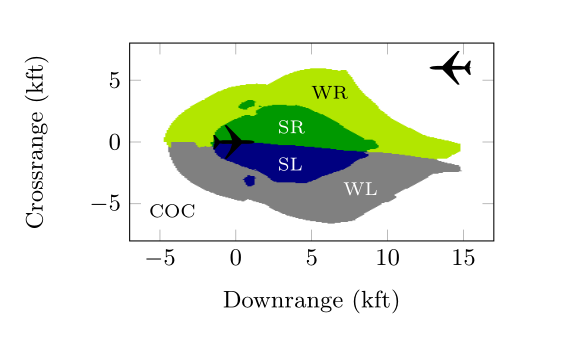
\includegraphics[width=1\linewidth]{13.png}
% 			\end{figure}
% 		\end{column}
% 	\end{columns}
% \end{frame}

\begin{frame}
	modify the assignments of variables: first pivot
	\begin{itemize}
		\item $T$:  regarded as a matrix expressing each of the basic
		variables (variables in $\mathcal{B}$) as a linear combination of non-basic variables (variables
		in $\mathcal{X} / \mathcal{B}$)
		\item $pivot(T, i, j)$: $x_{i}=\sum_{x_{k} \notin \mathcal{B}} c_{k} x_{k} \to x_{j}=\frac{x_{i}}{c_{j}}-\sum_{x_{k} \notin \mathcal{B}, k \neq j} \frac{c_{k}}{c_{j}} x_{k}$ 
		\item pivot step is switching of a basic variable $x_i$ (the leaving variable) with a non-basic variable
		$x_j$ (the entering variable)
	\end{itemize}
\end{frame}


\begin{frame}
	modify the assignments of variables: then update $(\alpha, x_j , \delta)$
	\begin{itemize}
		\item non-basic variables: $\alpha^{\prime}\left(x_{j}\right)=\alpha\left(x_{j}\right)+\delta$,else unchanged
		\item basic variables: $\alpha^{\prime}\left(x_{i}\right)=\alpha\left(x_{i}\right)+\delta \cdot T_{i, j}$
	\end{itemize}


\end{frame}

\begin{frame}
	\begin{columns}
		\begin{column}{.65\textwidth}
			\begin{figure}[htbp]
				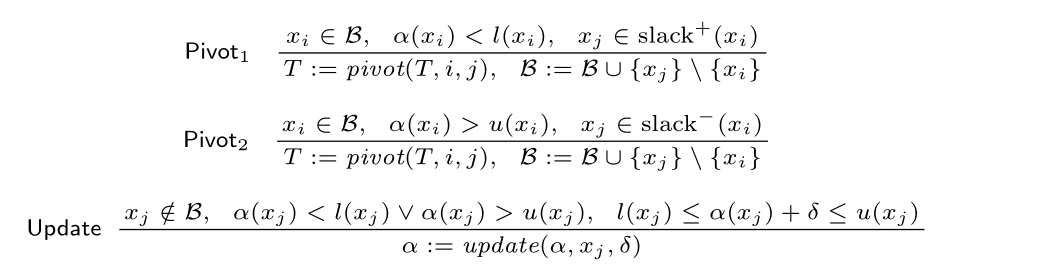
\includegraphics[width=1\linewidth]{1.png}
			\end{figure}

			\begin{figure}[htbp]
				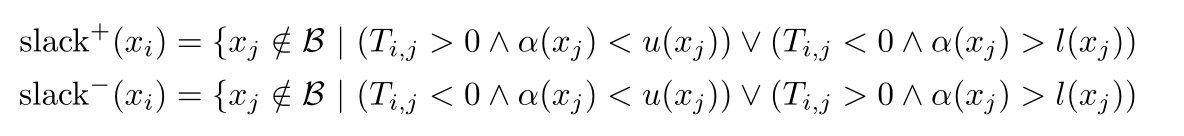
\includegraphics[width=1\linewidth]{2.png}
			\end{figure}
		\end{column}

		\begin{column}{.35\textwidth}
			\begin{itemize}
				\item slack: $x_j~\text{affords slack} \to x_i \text{closer to bound}$
				\item $+,-$ :assignment increse or decrease
			\end{itemize}
		\end{column}
	\end{columns}
\end{frame}


\begin{frame}
	\begin{figure}[htbp]
		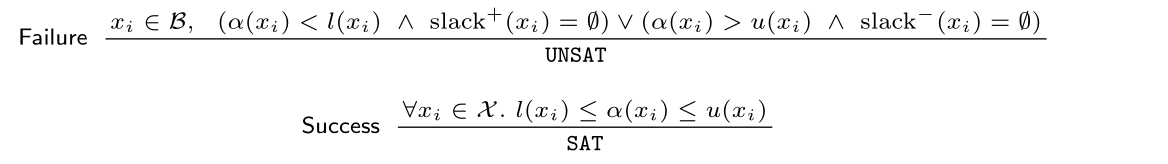
\includegraphics[width=1\linewidth]{3.png}
	\end{figure}
	Simplex allows variables to temporarily violate their bounds as it iteratively looks for a feasible variable assignment
\end{frame}


\section{Reluplex}
\begin{frame}
	\frametitle{Relu + Linear Real Arithmetic}
	How to adapt simplex to DNN 
	\begin{itemize}
		\item n nodes $\to 2^n$ conditions
		\item this theoretical worst-case behavior is also seen in practice	
	\end{itemize}
\end{frame}

\begin{frame}
	$\mathcal{T}_{\mathbb{R}} \to \mathcal{T}_{\mathbb{R} R}$:
	\begin{itemize}
		\item Signature: additionally includes the binary predicate \textbf{ReLU} with the interpretation:$ReLU(x, y) \iff y =\max(0, x)$
		\item Formulas: either linear inequalities or applications of the ReLU predicate to linear terms
	\end{itemize}
\end{frame}


\begin{frame}
	\begin{columns}
		\begin{column}{.65\textwidth}
			\begin{figure}[htbp]
				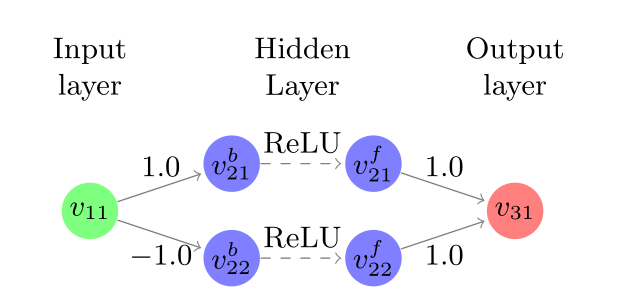
\includegraphics[width=1\linewidth]{4.png}
			\end{figure}
		\end{column}

		\begin{column}{.35\textwidth}
			Modify Relu nodes:
			\begin{itemize}
				\item Relu node $v \to v_b,v_f$
				\item assert $Relu(v_b,v_f)$
			\end{itemize}
		\end{column}
	\end{columns}
\end{frame}

\begin{frame}
	\frametitle{Reluplex}

	\begin{itemize}
		\item Reluplex also allows variables that are members of ReLU pairs to temporarily violate the ReLU semantics.
		\item and corrects them using \textbf{Pivot} and \textbf{Update} operations.
	\end{itemize}
	\begin{definition}[Reluplex configuration]
		\textbf{Reluplex configuration} is either \{SAT,UNSAT\} or a six-tuples $\langle\mathcal{B}, T, l, u,\alpha, R \rangle$:
		\begin{itemize}
			\item $\mathcal{B}, T, l, u,\alpha$ are as Simplex configuration
			\item $R \subset \mathcal{X} \times \mathcal{X}$ is the set of ReLU connections.
		\end{itemize}
	\end{definition}
	The \textbf{initial configuration} for a conjunction of atoms is also obtained as before except that $\langle x,y \rangle \in R$ iff $ReLU(x, y)$ is an atom.
\end{frame}

\begin{frame}
	\frametitle{Reluplex}
	\begin{itemize}
		\item Reluplex includes simplex transition rules \textbf{Pivot1}, \textbf{Pivot2} and \textbf{Update}, which are
		designed to handle out-of-bounds violations
		\item \textbf{Success} relu $\to$ \textbf{ReluSuccess} relu		
	\end{itemize}
	\begin{figure}[htbp]
		
\includegraphics[width=1\linewidth]{5.png}
	\end{figure}
	
\end{frame}

\begin{frame}
	\frametitle{Handling ReLU violations}
	\begin{columns}
		\begin{column}{.65\textwidth}
			\begin{figure}[htbp]
				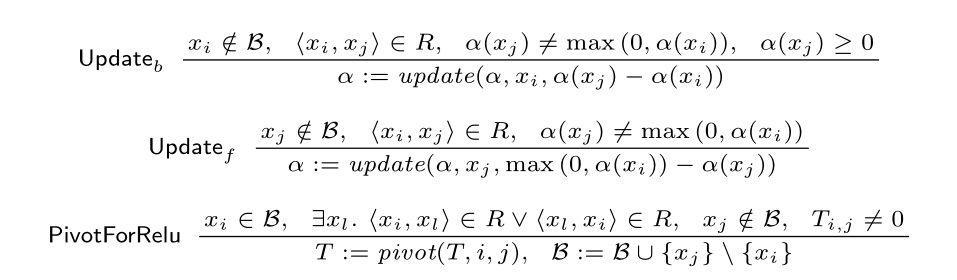
\includegraphics[width=1\linewidth]{6.png}
			\end{figure}
		\end{column}

		\begin{column}{.35\textwidth}
			\begin{itemize}
				\item  The \textbf{$Update_b$} and \textbf{$Update_f$} rules allow a broken ReLU connection to be
				corrected by updating the backward or forward-facing variables respectively
				\item  The \textbf{PivotForRelu} rule allows a basic variable appearing in a ReLU to be pivoted so that either \textbf{$Update_b$} or \textbf{$Update_f$} can be applied
			\end{itemize}
		\end{column}
	\end{columns}
\end{frame}

\begin{frame}
	\frametitle{ReluSplit}
	\begin{itemize}
		\item Split relu: $\textbf { ReluSplit } \frac{\left\langle x_{i}, x_{j}\right\rangle \in R, \quad l(x_{i})<0, \quad u(x_{i})>0}{u(x_{i}):=0~\vee~l(x_{i}):=0}$
		\item In practice, splitting can be managed by a SAT engine with \textbf{splitting-on-demand}
		\item Naive approach: applying the ReluSplit rule eagerly until it no longer applies and then solving each derived sub-problem separately
		\item Efficient approach: keep updating until the number of updates to a specific ReLU pair exceeds some threshold
	\end{itemize}

\end{frame}


\begin{frame}
	\frametitle{Example}
	\begin{columns}
		\begin{column}{.5\textwidth}
			\begin{figure}[htbp]
				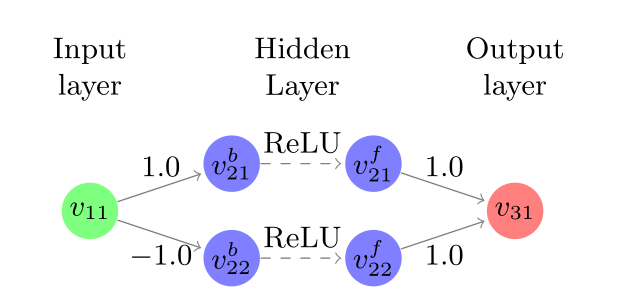
\includegraphics[width=1\linewidth]{4.png}
			\end{figure}
		\end{column}

		\begin{column}{.5\textwidth}
			\begin{itemize}
				\item Verify: $v_{11} \in[0,1] \text { and } v_{31} \in[0.5,1]$
				\item initial Relu configuration:
				\begin{equation}
					\left\{
						\begin{array}{lll}
						& a_{1}=-v_{11}+v_{21}^{b} \\
						& a_{2}=v_{11}+v_{22}^{b} \\
						& a_{3}=-v_{21}^{f}-v_{22}^{f}+v_{31}
					\end{array} \right.
				\end{equation}
				\item $\mathcal{B}=\left\{a_{1}, a_{2}, a_{3}\right\}, R = \left\{\left\langle v_{21}^{b}, v_{21}^{f}\right\rangle,\left\langle v_{22}^{b}, v_{22}^{f}\right\rangle\right\}$
				\item initial assignment:0; $l$ and $u$ of $\mathcal{B}:0$
				\item hidden variables:unbound,except $v_f$ are non negative
			\end{itemize}
		\end{column}
	\end{columns}
\end{frame}

\begin{frame}
	\frametitle{Example}
	\begin{columns}
		\begin{column}{.5\textwidth}
			\begin{figure}[htbp]
				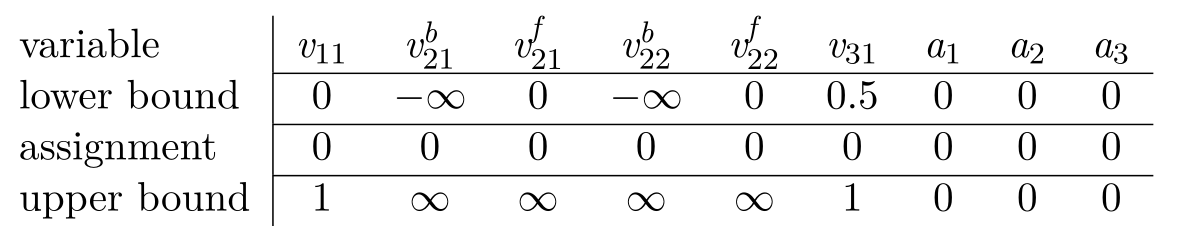
\includegraphics[width=1\linewidth]{7.png}
			\end{figure}
			\begin{figure}[htbp]
				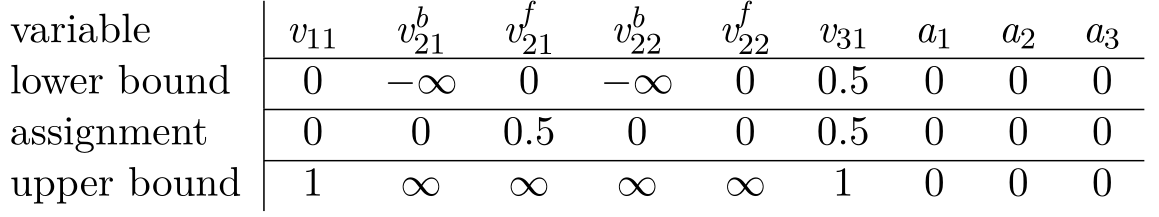
\includegraphics[width=1\linewidth]{8.png}
			\end{figure}
		\end{column}

		\begin{column}{.5\textwidth}
				First: fix any out-of-bounds variables.
			\begin{itemize}
				\item Update: $\alpha(v_{31}):0 \to 0.5,\alpha(a_{3}):0 \to 0.5$
				\item pivot: $a_{3}=-v_{21}^{f}-v_{22}^{f}+v_{31} \to v_{21}^{f}=-v_{22}^{f}+v_{31}-a_{3}$
				\item then update: $\alpha(a_{3}):0.5 \to 0,\alpha(v_{21}^f):0 \to 0.5$
				\item now tableau: 
				\begin{equation}
					\left\{
						\begin{array}{lll}
						& a_{1}=-v_{11}+v_{21}^{b} \\
						& a_{2}=v_{11}+v_{22}^{b} \\
						& v_{21}^{f}=-v_{22}^{f}+v_{31}-a_{3}
					\end{array} \right.
				\end{equation}
			\end{itemize}
		\end{column}
	\end{columns}
\end{frame}

\begin{frame}
	\frametitle{Example}
	\begin{columns}
		\begin{column}{.45\textwidth}
			\begin{figure}[htbp]
				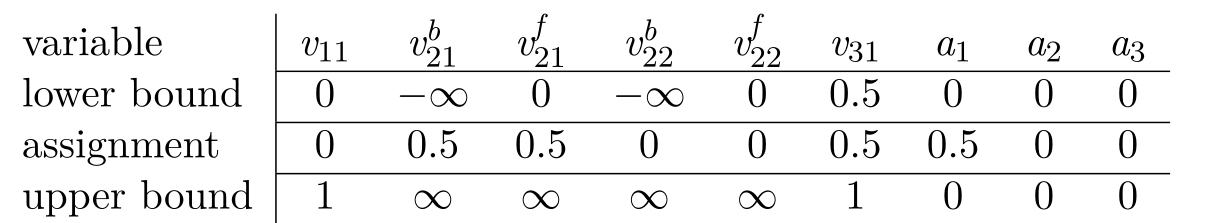
\includegraphics[width=1\linewidth]{9.png}
			\end{figure}
			\begin{figure}[htbp]
				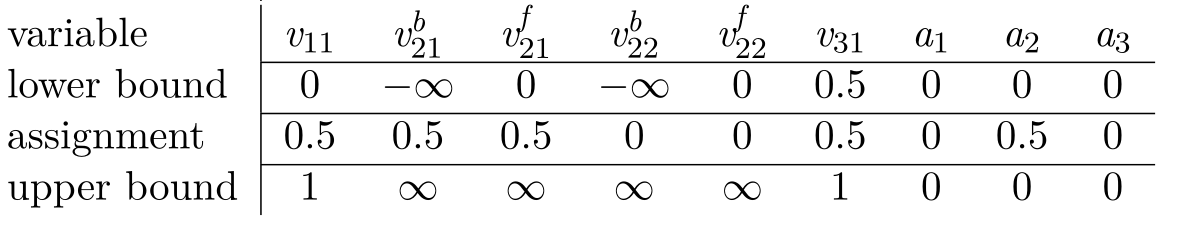
\includegraphics[width=1\linewidth]{10.png}
			\end{figure}
		\end{column}

		\begin{column}{.55\textwidth}
				Then: fix  the broken ReLU pair.
			\begin{itemize}
				\item $\alpha\left(v_{21}^{f}\right)=0.5 \neq 0=\max \left(0, \alpha\left(v_{21}^{b}\right)\right)$
				\item $Update_b$: $\alpha(v_{21}^b):0 \to 0.5,\alpha(a_{1}):0 \to 0.5$
				\item $\alpha(a_{1})$ is out of bound.
				\item pivot: $a_{1}=-v_{11}+v_{21}^{b} \to v_{11}=v_{21}^{b}-a_{1},a_{2}=v_{11}+v_{22}^{b} \to a_{2}=v_{21}^{b}+v_{22}^{b}-a_{1}$
				\item update: $\alpha(a_{1}):0.5 \to 0,\alpha(v_{11}):0 \to 0.5,\alpha(a_{2}):0 \to 0.5$
				% \item now tableau: 
				\begin{equation}
					\left\{
						\begin{array}{lll}
						& v_{11}=v_{21}^{b}-a_{1}\\
						& a_{2}=v_{21}^{b}+v_{22}^{b}-a_{1}\\
						& v_{21}^{f}=-v_{22}^{f}+v_{31}-a_{3}
					\end{array} \right.
				\end{equation}
			\end{itemize}
		\end{column}
	\end{columns}
\end{frame}

\begin{frame}
	\frametitle{Example}
	\begin{columns}
		\begin{column}{.5\textwidth}
			\begin{figure}[htbp]
				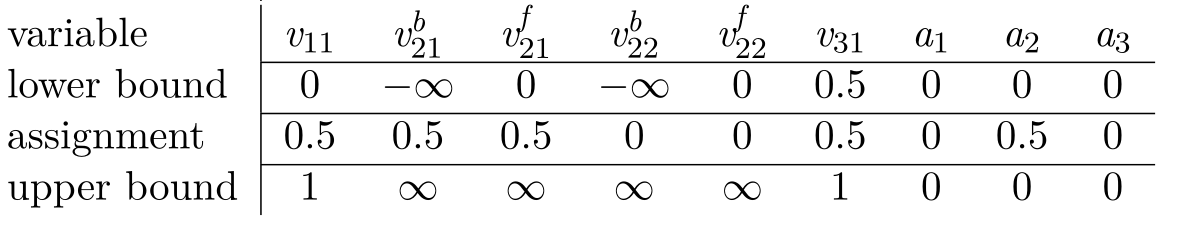
\includegraphics[width=1\linewidth]{10.png}
			\end{figure}
			\begin{figure}[htbp]
				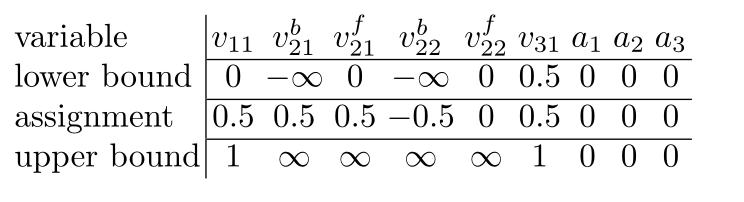
\includegraphics[width=1\linewidth]{11.png}
			\end{figure}
		\end{column}

		\begin{column}{.5\textwidth}
				Iteratively fix out-of-bounds variables.
			\begin{itemize}
				\item $\alpha(a_{2})$ is out of bound.
				\item pivot: $a_{2}=v_{21}^{b}+v_{22}^{b}-a_{1} \to v_{22}^{b}=-v_{21}^{b}+a_{1}+a_{2}$ 
				\item update: $\alpha(a_{2}):0.5 \to 0,\alpha(v_{22}^{b}):0 \to -0.5$
				% \item now tableau: 
				\begin{equation}
					\left\{
						\begin{array}{lll}
						& v_{11}=v_{21}^{b}-a_{1}\\
						& v_{22}^{b}=-v_{21}^{b}+a_{1}+a_{2}\\
						& v_{21}^{f}=-v_{22}^{f}+v_{31}-a_{3}
					\end{array} \right.
				\end{equation}
			\end{itemize}
		\end{column}
	\end{columns}
\end{frame}

% \begin{frame}
% 	\begin{tabular}{l|ccccccccc} 
% 						  variable    & $v_{11}$ & $v_{21}^{b}$ & $v_{21}^{f}$ & $v_{22}^{b}$ & $v_{22}^{f}$ & $v_{31}$ & $a_{1}$ & $a_{2}$ & $a_{3}$ \\
% 		\cline { 2 - 10 } lower bound & 0        & $-\infty$    & 0            & $-\infty$    & 0            & $0.5$ & 0 & 0 & 0 \\
% 		\cline { 2 - 10 } assignment  & 0        & 0.5          & 0.5          & 0            & 0            & 0.5  & 0.5 & 0 & 0 \\
% 		\cline { 2 - 10 } upper bound & 1        & $\infty$     & $\infty$     & $\infty$     & $\infty$ & 1 & 0 & 0 & 0
% 	\end{tabular}

% 	\begin{tabular}{l|ccccccccc} 
% 		variable & $v_{11}$ & $v_{21}^{b}$ & $v_{21}^{f}$ & $v_{22}^{b}$ & $v_{22}^{f}$ & $v_{31}$ & $a_{1}$ & $a_{2}$ & $a_{3}$ \\
% 		\cline { 2 - 10 } lower bound & 0 & $-\infty$ & 0 & $-\infty$ & 0 & $0.5$ & 0 & 0 & 0 \\
% 		\cline { 2 - 10 } assignment & 0.5 & 0.5 & 0.5 & 0 & 0 & 0.5 & 0 & 0.5 & 0 \\
% 		\cline { 2 - 10 } upper bound & 1 & $\infty$ & $\infty$ & $\infty$ & $\infty$ & 1 & 0 & 0 & 0
% 	\end{tabular}

% \end{frame}

% \begin{frame}
% 	\begin{tabular}{c|ccccccccc}
% 		$\mathrm{T}$  & $p$  & $q$ & $r$ & $s$ & $t$ &   & $\mathrm{Ib}$ & $\beta$ & $u b$ \\
% 		\hline$x$     & $-2$ & 1   &     &     &         & 0             & $-1$    & 0 \\
% 		$y$           &      & 1   & 2   &     &         & 0             & 0       & 0 \\
% 		$z$ & & & $-1$ & 1 & 1 & 0 & 0 & 0 \\
% 		$u b$ & 1 & $+\infty$ & $+\infty$ & $+\infty$ & $+\infty$ & & & \\
% 		$\alpha$ & $0.5$ & 0 & 0 & 0 & 0 & & & \\
% 		$\mathrm{lb}$ & $0.5$ & $-\infty$ & $-\infty$ & 0 & 0 & & Simplex
% 		\end{tabular}
% \end{frame}


\section{ Efficiently Implementing Reluplex}

\begin{frame}
	\frametitle{Tighter Bound Derivation}
	\begin{itemize}
		\item $\operatorname{pos}\left(x_{i}\right)=\left\{x_{j} \notin \mathcal{B} \mid T_{i, j}>0\right\},\operatorname{neg}\left(x_{i}\right)=\left\{x_{j} \notin \mathcal{B} \mid T_{i, j}<0\right\}$
		\item Throughout the execution, the following rules can be used to derive tighter bounds for $x_i$, regardless of the current assignment:
			$$\text { deriveLowerBound } \frac{x_{i} \in \mathcal{B}, \quad l\left(x_{i}\right)<\sum_{x_{j} \in \operatorname{pos}\left(x_{i}\right)} T_{i, j} \cdot l\left(x_{j}\right)+\sum_{x_{j} \in \operatorname{neg}\left(x_{i}\right)} T_{i, j} \cdot u\left(x_{j}\right)}{l\left(x_{i}\right):=\sum_{x_{j} \in \operatorname{pos}\left(x_{i}\right)} T_{i, j} \cdot l\left(x_{j}\right)+\sum_{x_{j} \in \operatorname{neg}\left(x_{i}\right)} T_{i, j} \cdot u\left(x_{j}\right)}$$\\
			$$\text { deriveUpperBound } \frac{x_{i} \in \mathcal{B}, \quad u\left(x_{i}\right)>\sum_{x_{j} \in \operatorname{pos}\left(x_{i}\right)} T_{i, j} \cdot u\left(x_{j}\right)+\sum_{x_{j} \in \operatorname{neg}\left(x_{i}\right)} T_{i, j} \cdot l\left(x_{j}\right)}{u\left(x_{i}\right):=\sum_{x_{j} \in \operatorname{pos}\left(x_{i}\right)} T_{i, j} \cdot u\left(x_{j}\right)+\sum_{x_{j} \in \operatorname{neg}\left(x_{i}\right)} T_{i, j} \cdot l\left(x_{j}\right)}$$
		\item contribute to fix the active or inactive state, without splitting
	\end{itemize}
\end{frame}

\begin{frame}
	\frametitle{Derived Bounds and Conflict Analysis}
	\begin{itemize}
		\item Bound derivation can lead to situations: $l(x) > u(x)$
		\item Such contradictions allow Reluplex to immediately undo a previous split (or answer \textbf{UNSAT} if no previous splits exist). 
		\item Use \emph{Conflict Analysis}: in many cases more than just the previous split can be undone
	\end{itemize}
\end{frame}

% \begin{frame}
% 	\frametitle{Floating Point Arithmetic}
% 	\begin{itemize}
% 		\item Scalability:use floating point arithmetic instead of precise arithmetic
% 		\item Such contradictions allow Reluplex to immediately undo a previous split (or answer \textbf{UNSAT} if no previous splits exist). 
% 		\item Use \emph{Conflict Analysis}: in many cases more than just the previous split can be undone
% 	\end{itemize}
% \end{frame}



\section{Experiments}
\begin{frame}
	\frametitle{ACAS Xu(Airborne Collision Avoidance System X unmanned)}
	\begin{figure}
		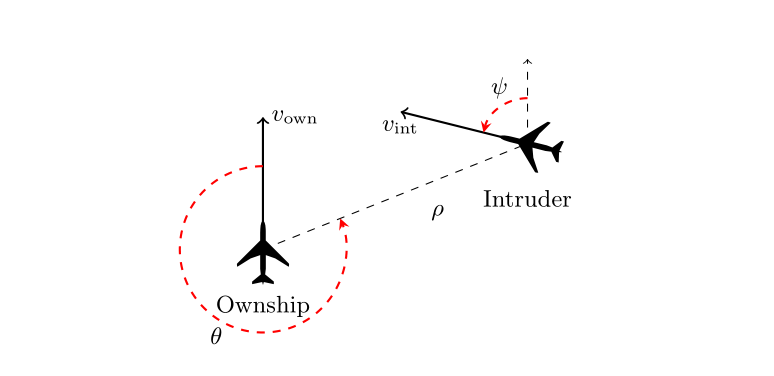
\includegraphics[width=0.75\linewidth]{12.png}
	\end{figure}
\end{frame}

\begin{frame}
	\frametitle{Prove Network Properties}
	\begin{figure}
		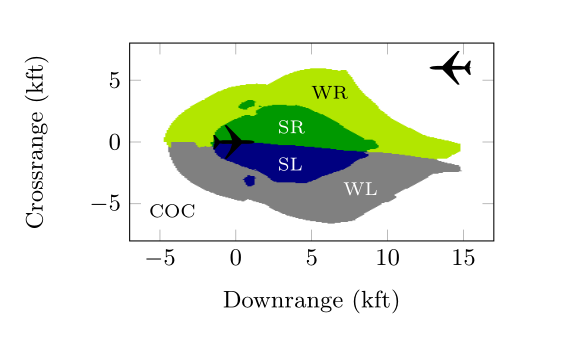
\includegraphics[width=0.75\linewidth]{13.png}
	\end{figure}

	\begin{itemize}
		\item The system does not give unnecessary turning advisories
		\item Alerting regions are uniform and do not contain inconsistent alerts
		\item Strong alerts do not appear for high vertical separation values.
	\end{itemize}
\end{frame}

\begin{frame}
	\frametitle{Evaluation}
	Search strategy:
	\begin{itemize}
		\item First repeatedly fix any out-of-bounds violations
		\item Then correct any violated ReLU constraints( possibly introducing new out-of-bounds violations) 
		\item Perform bound tightening on the entering variable after every pivot operation,and perform a more thorough bound tightening on all the equations in the tableau once every few thousand pivot steps.
	\end{itemize}

\end{frame}

\begin{frame}
	\frametitle{Results}
	\begin{figure}
		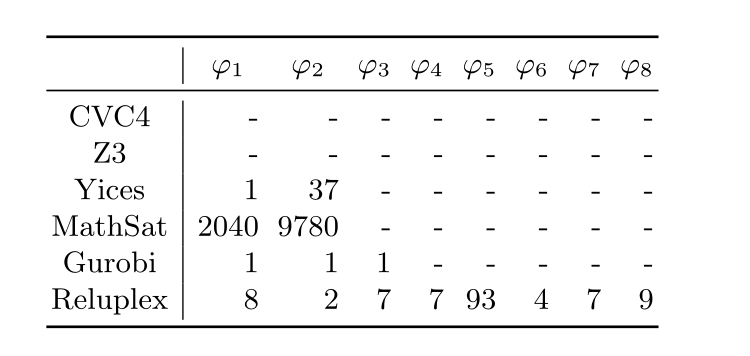
\includegraphics[width=0.75\linewidth]{14.png}
	\end{figure}
\end{frame}

\begin{frame}
	\frametitle{Results}
	\begin{figure}[htbp]
		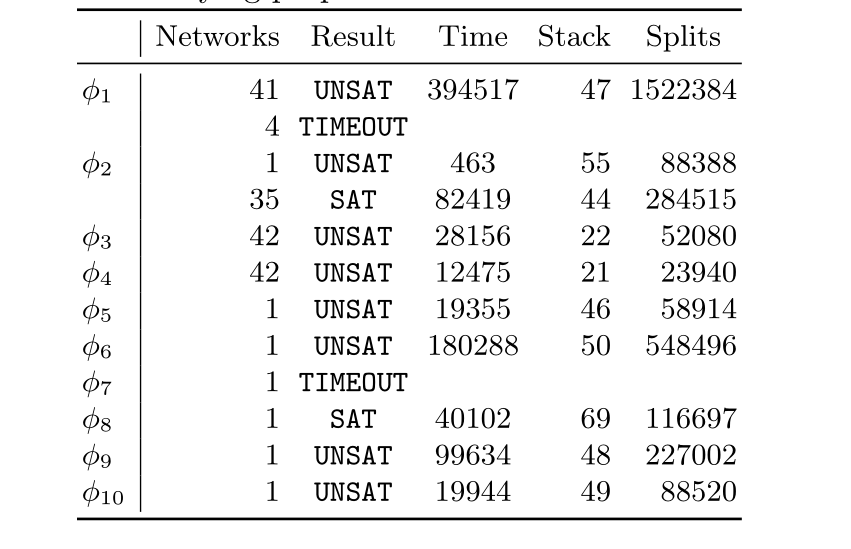
\includegraphics[width=0.4\linewidth]{15.png}
	\end{figure}

	\begin{itemize}
		\item Stack:maximal depth of nested case-splits reached
		\item Splits:total number of case-splits performed
	\end{itemize}
\end{frame}

\begin{frame}
	\frametitle{Robustness}
	\begin{figure}
		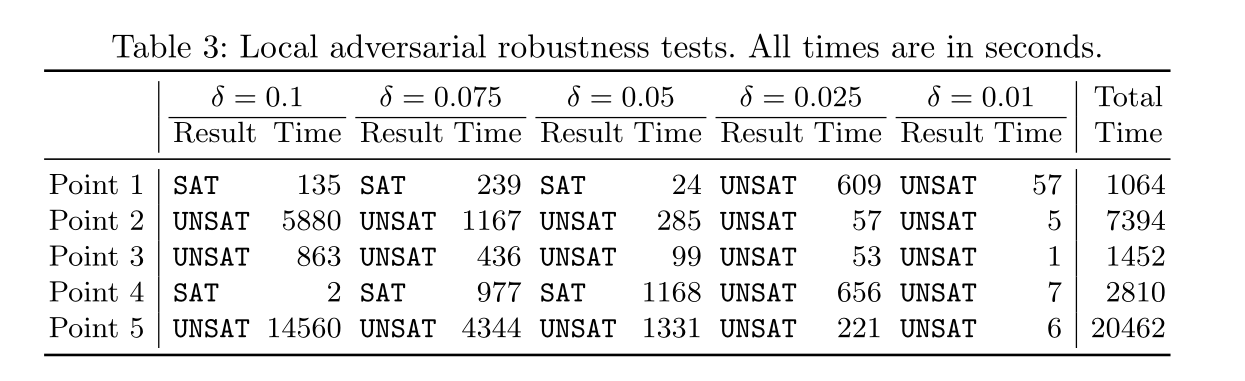
\includegraphics[width=0.75\linewidth]{16.png}
	\end{figure}

	\begin{itemize}
		\item \emph{$\delta$-locally-robust} at input point $x$ 
		\item \emph{$\epsilon$-globally-robust}:only on small networks;improving the
		scalability of this technique is left for future work.
	\end{itemize}
\end{frame}
%------------------------------------------------


%------------------------------------------------

%------------------------------------------------


%------------------------------------------------
\begin{frame}
\hfill
\center{\Huge{\calligra{\Huge{Thank you}}}}
\linespread{3}\selectfont
\end{frame}
%----------------------------------------------------------------------------------------
\end{document}